\section{Link Budget}

To generate the synthetic signal, the EIRP of transmitted signal is verified by link budget analysis.
\begin{table}[]
\centering
\caption{Link budget}
\label{table: link_budget}
\begin{tabular}{lrl}
\hline
Frequency                        & 260.375    & MHz \\ \hline
Bandwidth                        & 25         & kHz \\ \hline
EIRP                             & 26         & dBW \\ \hline
Fading loss                      & 6          & dB  \\ \hline
Elevation angle                  & 40         & deg \\ \hline
Distance                         & 37780.2664 & km  \\ \hline
Space loss along direct path     & 162.5374   & dB  \\ \hline
Effective area isotropic antenna & 9.7677     & dB  \\ \hline
Received power                   & -152.3051  & dBW \\ \hline
Noise power                      & -159.9958  & dBW \\ \hline
SNR input                        & 7.6907     & dB  \\ \hline
System noise figure              & 1.6994     & dB  \\ \hline
SNR output                       & 5.9913     & dB  \\ \hline
\end{tabular}
\end{table}

\section{Measurement Simulation}

To verify the measurement theory, we establish a comprehensive simulator from  satellites to receiver with Matlab. The simulator includes signal resource, path ray of transmitted signal, antenna gain, and receiver parameters.

\subsection{Synthetic Signal}
There are multiple channels transmitted by satellites. At the first step, we consider one satellite with $N$ channels, and the received discrete signal composed with $N$ channels is defined by
\begin{equation}
x_D[n] = \sum_{i=1}^N \sqrt{C_{D,i}} a_i [n-\tau_D^s]e^{j ((\omega_{c,i} - \omega_I) \frac{n}{f_s}+\omega_{c,i} \tau_D)}
\end{equation}
Where $C$ is the carrier power from path loss model, $a$ denotes the modulation, $\tau$ is the delay due to the distance between the satellite and the receiver, $\tau^s$ is the delay in sample, $\omega_c$ is the carrier frequency in radians, $\omega_I$ is the intermediate frequency, $f_s$ is the sampling rate, and $i$ are $D$ represents the $i^{th}$ channel and received signal along direct path ray.  The range of $\omega_c$ is limited by the sampling rate. The delay depends on the the geometry of the satellites and the receiver. The carrier power $C$ is calculated by
\begin{equation}
C_{D,i}=EIRP \frac{1}{4 \pi d^2} \frac{\lambda_i^2}{4 \pi}
\end{equation}
Where the transmitted power at the satellite is defined by Equivalent Isotropically Radiated Power (EIRP), $d$ is the distance between the satellite and receiver, and $\lambda_i$ is the delay of the $i^{th}$ channel. The modulation of signal is set to quadrature phase-shift keying (QPSK), and the discrete signal is expressed as
\begin{equation}
a_i[n] =  \sum_{q=0}^{N-1} rect (\frac{n-(q+1/2)n_c}{n_c})e^{j (2 \mathcal{U}_q +1) \frac{\pi}{4} }
\end{equation}
Where $\mathcal{U}_q$ is uniform distribution with integers 0, 1, 2, and 3,  $T_c$ is the chipping time, $T_s$ is the sampling time, and $n_c$ is the number of samples within one chip. We consider the chipping time is equal to $\frac{1}{bw}$.The reflect signal is
\begin{equation}
x_R[n] = \sum_{i=1}^N \sqrt{C_{R,i}} a_i [n-\tau_{R,i}^s]e^{j ((\omega_{c,i} - \omega_I) \frac{n}{f_s}+\omega_{c,i} \tau_{R})}
\end{equation}
$C_{R,i}$ denotes the carrier power of reflect signal, and it is given by
\begin{equation}
C_{R,i} = \Gamma C_{D,i}
\end{equation}
Where $\Gamma$ is the reflectivity at the specular point of the satellite. The delay along reflect path ray is obtained by
\begin{equation}
\tau_{R} = \tau_{D} +  \frac{2 h sin \theta}{c}
\end{equation}
Where $h$ is the altitude above the specular point, $\theta$ denotes the elevation angle, and $c$ is the speed of light. If two satellites transmitted signals within the same frequency range, the delay, elevation, and reflectivity can be different according to the geometry of satellites. Figure \ref{fig:simu_xDxR} shows the synthetic signals of two satellites, and the sampling rate is 8.5 MHz. The left and right columns are the synthetic signals along direct and reflect path rays, and the figures of the first and second rows  are the signals for the individual satellites 1 and 2. The figures in the last row shows the synthetic signals from both satellites at the same time.
\begin{figure}[t!]
	\centering
	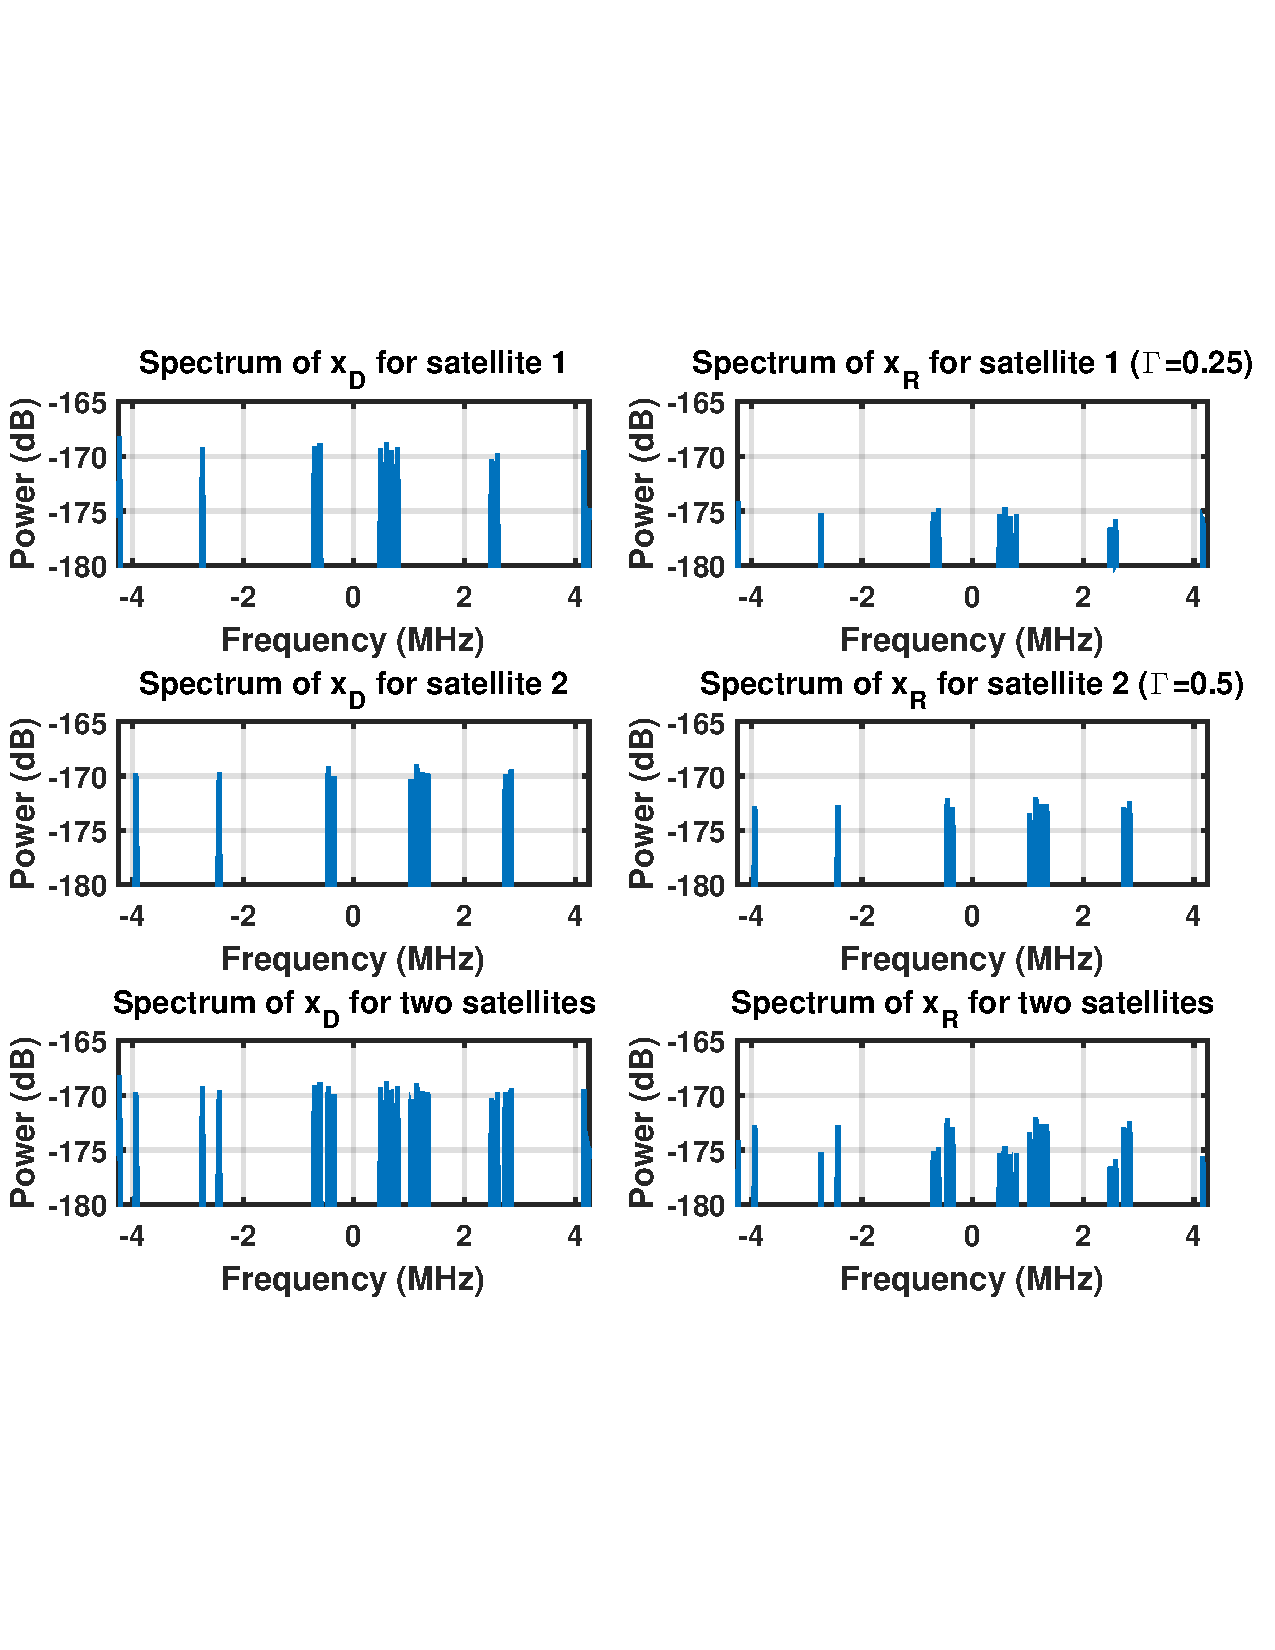
\includegraphics[width=4in]{pdf/Simulator_xDxR.pdf}
	\caption{The synthetic signals from different satellites; the left and right columns are for $x_D$ and $x_R$, and the first, second, and third rows are for satellite 1, 2, and both satellites. }
	\centering
	\label{fig:simu_xDxR}
\end{figure}
The complete received signal includes antenna gain, channel gain, and thermal noise from antenna and receiver. The antenna gain depends on the attitude of receiver, and the difference cross the channels is ignored. The expression of received signal for two channels for T-State are
\begin{equation}
\begin{bmatrix}x^T_1[n] \\ x^T_2[n] \end{bmatrix} = 
\begin{bmatrix}\sqrt{G_1} & 0 \\ 0 & \sqrt{G_2} \end{bmatrix} 
\begin{bmatrix}\sqrt{G_{S,D}} & \sqrt{G_{S,R}}  \\ \sqrt{G_{E,D}} & \sqrt{G_{E,R}} \end{bmatrix} 
\begin{bmatrix}x_D[n] \\ x_R[n] \end{bmatrix} +
\begin{bmatrix} n_{pre,S}[n] \\ n_{pre,E}[n] \end{bmatrix} + 
\begin{bmatrix} n_{post,1}[n] \\ n_{post,2}[n] \end{bmatrix} 
\end{equation}
Where $\mathcal{N}(\mu, \sigma)$ represents a random variable of Gaussian distribution with mean $\mu$ and standard deviation $\sigma$. Once the receiver switches to S-State, the received signals become
\begin{equation}
\begin{bmatrix}x^S_1[n] \\ x^S_2[n] \end{bmatrix} = 
\begin{bmatrix}\sqrt{G_2} & 0 \\ 0 & \sqrt{G_1} \end{bmatrix} 
\begin{bmatrix}\sqrt{G_{S,D}} & \sqrt{G_{S,R}}  \\ \sqrt{G_{E,D}} & \sqrt{G_{E,R}} \end{bmatrix} 
\begin{bmatrix}x_D[n] \\ x_R[n] \end{bmatrix} +
\begin{bmatrix} n_{pre,S}[n] \\ n_{pre,E}[n] \end{bmatrix} + 
\begin{bmatrix} n_{post,1}[n] \\ n_{post,2}[n] \end{bmatrix} 
\end{equation}
When the calibration state moves to C-state
\begin{equation}
\begin{bmatrix}x^C_1[n] \\ x^C_2[n] \end{bmatrix} = 
\begin{bmatrix}x^T_1[n] \\ x^T_2[n] \end{bmatrix} +
\begin{bmatrix}1 \\ 1 \end{bmatrix}n_{cal}[n]
\end{equation}
And the last state is R-state
\begin{equation}
\begin{bmatrix}x^R_1[n] \\ x^R_2[n] \end{bmatrix} = 
\begin{bmatrix} n_{ref,1}[n] \\ n_{ref,2}[n] \end{bmatrix}  +
\begin{bmatrix} n_{post,1}[n] \\ n_{post,2}[n] \end{bmatrix} 
\end{equation}\subsection{Signal processing of synthetic signal}
To process specific single channel, the synthetic signals need to be shifted to the targeted channel ($\omega_c$) and applied the narrow band filter. 
\begin{equation}
\begin{bmatrix}x_1[n,\omega_c] \\ x_2[n,\omega_c] \end{bmatrix} = \sum_{m=0}^{m=T_I f_s} (
\begin{bmatrix}x_1[m] \\ x_2[m] \end{bmatrix} 
e^{-j ((\omega_{c} - \omega_I) \frac{m}{f_s}} f_{lp}[n-m])
\end{equation}
Where $f_{lp}$  is the impulse response of the narrow band low pass filter, and it is applied by the discrete convolution . The correlators include the autocorrelation of  $x_1$, autocorrelation of $x_2$, and cross-correlation of $x_1$ and $x_2$ with five lags ($\tau^s_1$, $\tau^s_2$, $\tau^s_3$,$\tau^s_4$, and $\tau^s_5$), and they are 0, $\tau^s_{RD} - \frac{n_c}{8}$,  $\tau^s_{RD} $, $\tau^s_{RD} +\frac{n_c}{8}$, and $\tau^s >> n_c$. The correlations are denoted by
\begin{align}
Y_{11}(\tau^s_i) &= \frac{1}{T_I f_s}\sum_{m=0}^{m=T_I f_s} x_1[m] x^*_1[m+\tau^s_i]  \\
Y_{12}(\tau^s_i) &=  \frac{1}{T_I f_s}\sum_{m=0}^{m=T_I f_s} x_1[m] x^*_2[m+\tau^s_i] \\
Y_{22}(\tau^s_i) &=  \frac{1}{T_I f_s}\sum_{m=0}^{m=T_I f_s} x_2[m] x^*_2[m+\tau^s_i]
\end{align}

\begin{figure}[t!]
	\centering
	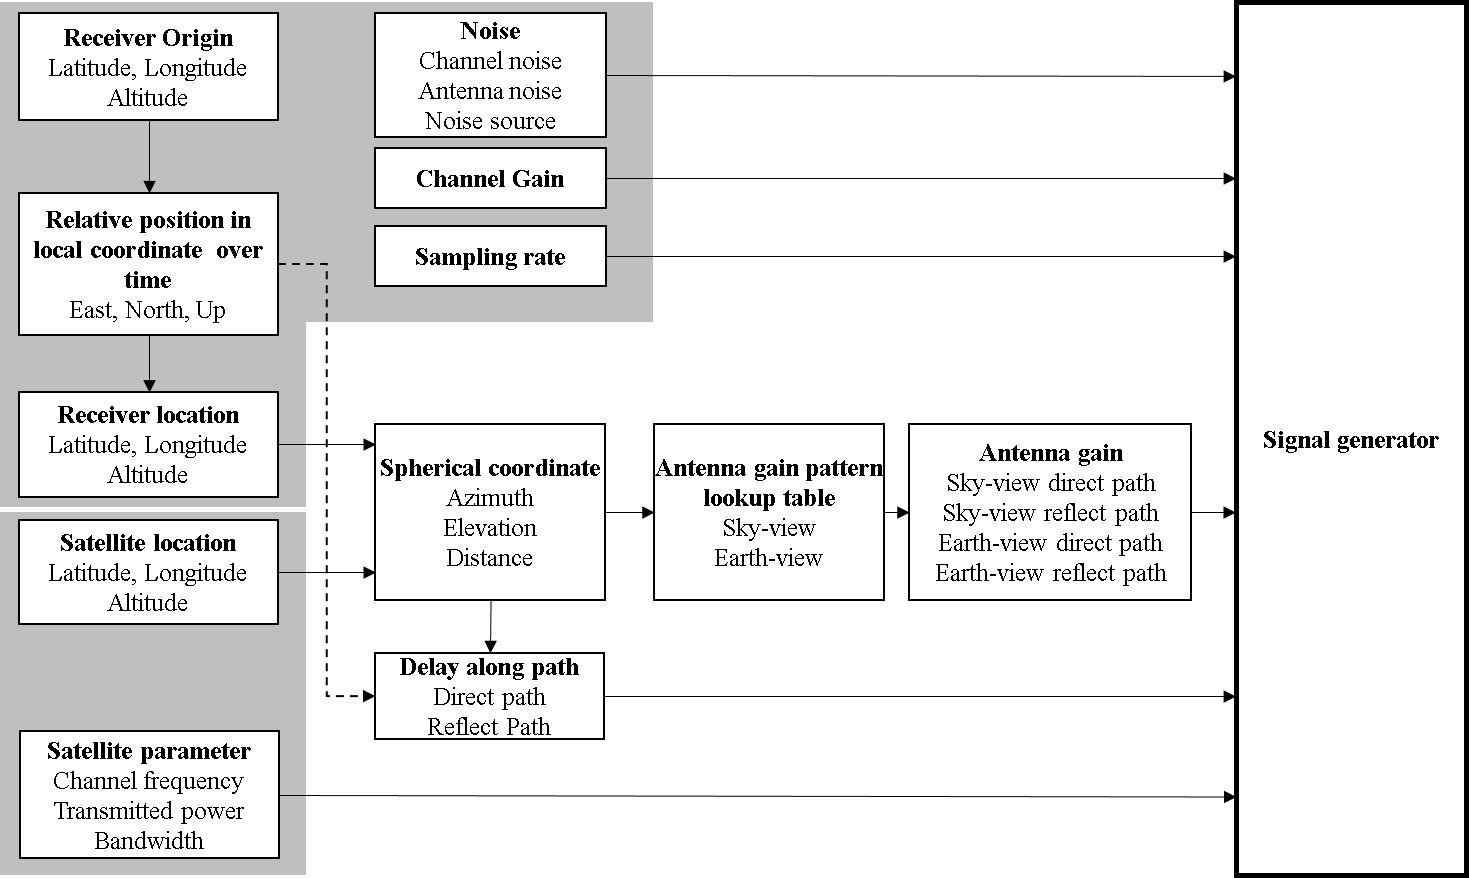
\includegraphics[width=4in]{pdf/simu_chart1.jpg}
	\caption{The flow chart of simulator }
	\centering
	\label{fig:Simu_flow_chart}
\end{figure}
\begin{figure}[t!]
	\centering
	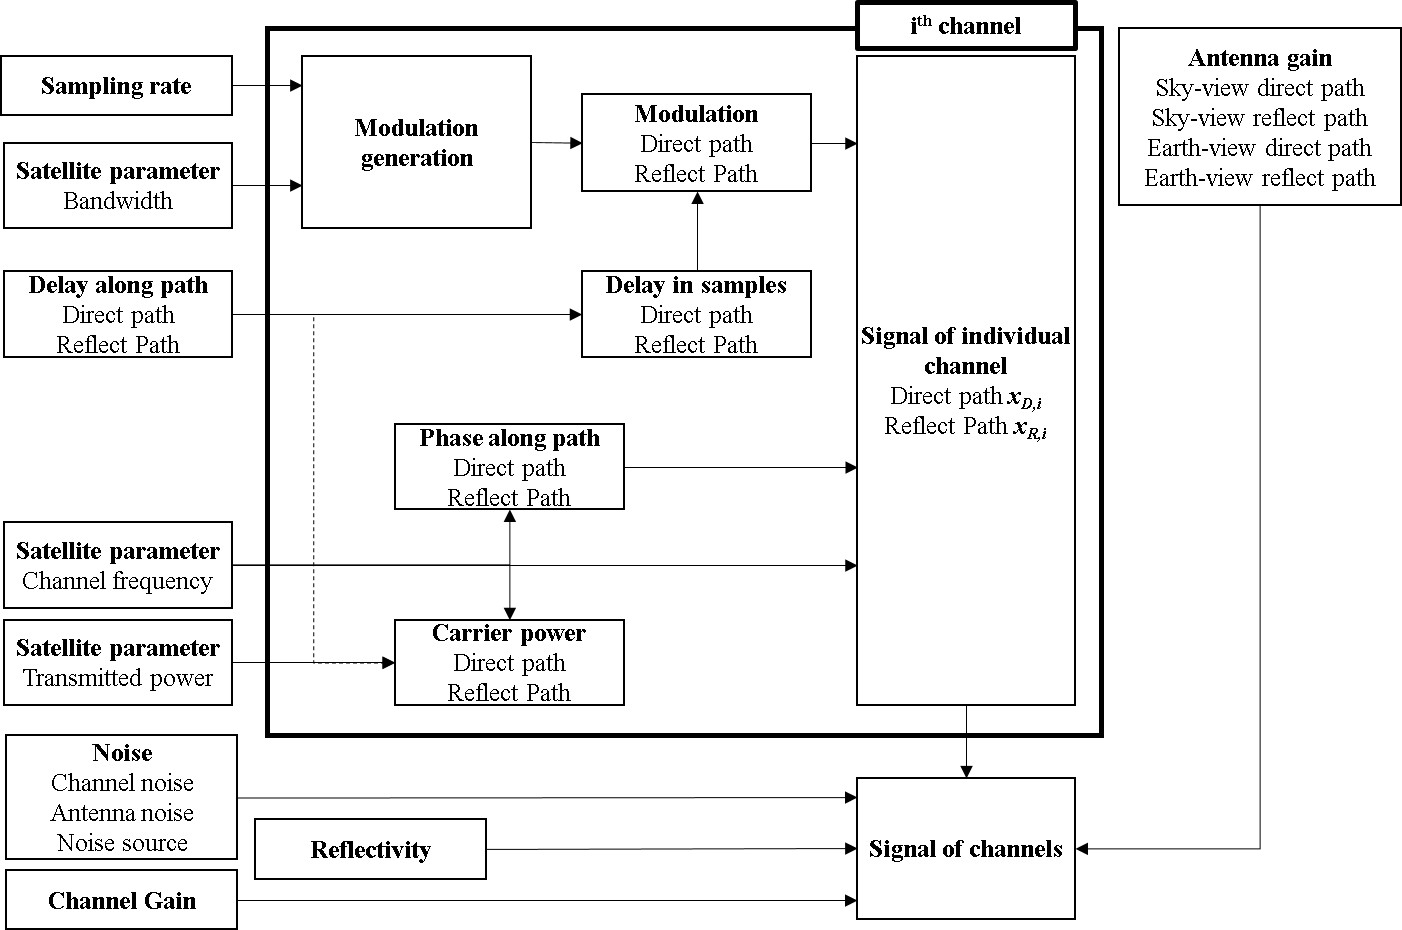
\includegraphics[width=4in]{pdf/simu_chart2.jpg}
	\caption{The flow chart of simulator. }
	\centering
	\label{fig:Simu_flow_chart}
\end{figure}
